\documentclass[10pt]{article}

% Packages and macros go here
\usepackage[T1]{fontenc}
\usepackage{lmodern}
\usepackage[utf8x]{inputenx}
\usepackage{microtype}
\usepackage{framed}
\usepackage{listings}
\usepackage{vmargin}
\usepackage{setspace}
\usepackage{mathrsfs, mathenv}
\usepackage{amsmath, amsthm, amssymb, amsfonts, amscd}
\usepackage{graphicx}
\usepackage{epstopdf}
\usepackage[svgnames]{xcolor}
\usepackage{hyperref}
\usepackage[capitalise]{cleveref}
\hypersetup{citecolor=blue, colorlinks=true, linkcolor=black}
\setlength{\parskip}{6pt}
\setlength\parindent{0pt}
\usepackage{subcaption}
\usepackage{bbm}
\usepackage{cite}
\usepackage{verbatim}
\usepackage{pgfplots}
\usepackage{tikz}
\usepackage{etoolbox}
\usepackage{color}
\usepackage{lipsum}
\usepackage{ifthen}
\usepackage[linesnumbered, ruled, vlined]{algorithm2e}
\crefname{algocf}{Algorithm}{Algorithms}
\usepackage{autonum}

\theoremstyle{plain}
\newtheorem{theorem}{Theorem}[section]
\newtheorem{corollary}[theorem]{Corollary}
\newtheorem{lemma}[theorem]{Lemma}
\newtheorem{proposition}[theorem]{Proposition}
\numberwithin{equation}{section}

\theoremstyle{definition}
\newtheorem{definition}[theorem]{Definition}

\theoremstyle{remark}
\newtheorem{remark}[theorem]{Remark}
\newtheorem{assumption}[theorem]{Assumption}
\newtheorem{example}[theorem]{Example}


\ifpdf
  \DeclareGraphicsExtensions{.eps,.pdf,.png,.jpg}
\else
  \DeclareGraphicsExtensions{.eps}
\fi

\usepackage{mathtools}
% basics

% tables
\usepackage{booktabs}

% plots
\usepackage{pgfplots}
\usepackage{tikz}
\usetikzlibrary{patterns,arrows,decorations.pathmorphing,backgrounds,positioning,fit,matrix}
\usepackage[labelfont=bf]{caption}
\setlength{\belowcaptionskip}{-5pt}
\usepackage{here}
\usepackage[font=normal]{subcaption}

% Prevent itemized lists from running into the left margin inside theorems and proofs
\usepackage{enumitem}
\setlist[itemize]{leftmargin=.5in}
\setlist[enumerate]{leftmargin=.5in,topsep=3pt,itemsep=3pt,label=(\roman*)}

% Add a serial/Oxford comma by default.
\newcommand{\creflastconjunction}{, and~}

% Sets running headers as well as PDF title and authors
% title and authors

\newcommand{\email}[1]{\href{#1}{#1}}
\newcommand{\TheTitle}{Probabilistic methods for elliptic partial differential equations} 
\newcommand{\TheAuthors}{A. Abdulle, G. Garegnani}
%\headers{Random time steps for quantifying chaotic numerical integration}{\TheAuthors}
\title{{\TheTitle}}
\newcommand*\samethanks[1][\value{footnote}]{\footnotemark[#1]}
\author{Assyr Abdulle\thanks{Institute of Mathematics, \'Ecole Polytechnique F\'ed\'erale de Lausanne (\email{\{assyr.abdulle, giacomo.garegnani\}@epfl.ch})}
	\and
	Giacomo Garegnani\samethanks}
\date{}

\usepackage{amsopn}
\DeclareMathOperator{\diag}{diag}
\DeclarePairedDelimiter{\ceil}{\left\lceil}{\right\rceil}
\DeclarePairedDelimiter{\floor}{\lfloor}{\rfloor}
\DeclarePairedDelimiter{\abs}{\lvert}{\rvert}
\DeclarePairedDelimiter{\norm}{\lVert}{\rVert}
\renewcommand{\phi}{\varphi}
\renewcommand{\theta}{\vartheta}
\renewcommand{\Pr}{\mathbb{P}}
\newcommand{\btilde}{\widetilde}
\newcommand{\bhat}{\widehat}
\newcommand{\eqtext}[1]{\ensuremath{\stackrel{#1}{=}}}
\newcommand{\leqtext}[1]{\ensuremath{\stackrel{#1}{\leq}}}
\newcommand{\iid}{\ensuremath{\stackrel{\text{i.i.d.}}{\sim}}}
\newcommand{\totext}[1]{\ensuremath{\stackrel{#1}{\to}}}
\newcommand{\rightarrowtext}[1]{\ensuremath{\stackrel{#1}{\longrightarrow}}}
\newcommand{\leftrightarrowtext}[1]{\ensuremath{\stackrel{#1}{\longleftrightarrow}}}
\newcommand{\pdv}[2]{\ensuremath\partial_{#2}#1}
\newcommand{\N}{\mathbb{N}}
\newcommand{\R}{\mathbb{R}}
\newcommand{\C}{\mathbb{C}}
\newcommand{\OO}{\mathcal{O}}
\newcommand{\epl}{\varepsilon}
\newcommand{\diffL}{\mathcal{L}}
\newcommand{\prior}{\mathcal{Q}}
\newcommand{\defeq}{\coloneqq}
\newcommand{\eqdef}{\eqqcolon}
\newcommand{\Var}{\operatorname{Var}}
\newcommand{\E}{\operatorname{\mathbb{E}}}
\newcommand{\MSE}{\operatorname{MSE}}
\newcommand{\trace}{\operatorname{tr}}
\newcommand{\MH}{\mathrm{MH}}
\newcommand{\ttt}{\texttt}
\newcommand{\Hell}{d_{\mathrm{H}}}
\newcommand{\sksum}{{\textstyle\sum}}
\newcommand{\dd}{\, \mathrm{d}}
\renewcommand{\d}{\mathrm{d}}
\definecolor{shade}{RGB}{100, 100, 100}
\definecolor{bordeaux}{RGB}{128, 0, 50}
\newcommand{\corr}[1]{{\color{red}#1}}
\newcommand{\Tau}{\tau}
\newcommand{\LL}{L}
\newcommand{\HH}{H}
\newcommand{\WW}{W}
\newcommand{\mbf}{\mathbf}
\newcommand{\bfs}{\boldsymbol}
\newcommand{\todo}{{\color{red} TO DO}}
\newcommand{\X}{\mathbb{X}}
\newcommand{\nablar}{\nabla_{\hat x}}
\newcommand{\eval}[1]{\bigr\rvert_{#1}}
\newcommand{\normm}[1]{\norm{#1}_a}
%\newcommand{\normm}[1]{{\left\vert\kern-0.25ex\left\vert\kern-0.25ex\left\vert #1 
%		\right\vert\kern-0.25ex\right\vert\kern-0.25ex\right\vert}}

\usepackage[usestackEOL]{stackengine}
\newcommand\fop[3][9pt]{\mathop{\ensurestackMath{\stackengine{#1}%
			{\displaystyle#2}{\scriptstyle#3}{U}{c}{F}{F}{L}}}\limits}
\newcommand\finf[2][9pt]{\fop[#1]{\inf}{#2}}
\newcommand\fsum[2][14pt]{\fop[#1]{\sum}{#2}}

\definecolor{leg1}{RGB}{0,114,189}
\definecolor{leg2}{RGB}{217,83,25}
\definecolor{leg3}{RGB}{237,177,32}
\definecolor{leg4}{RGB}{126,47,142}
\definecolor{leg5}{RGB}{119,172,48}

\definecolor{leg21}{RGB}{62,38,169}
\definecolor{leg22}{RGB}{46,135,247}
\definecolor{leg23}{RGB}{55,200,151}
\definecolor{leg24}{RGB}{254,195,56}


\ifpdf
\hypersetup{
	pdftitle={\TheTitle},
	pdfauthor={\TheAuthors}
}
\fi


\begin{document}
\maketitle	

\begin{abstract}
	
\end{abstract}

\textbf{AMS subject classification.}

\textbf{Keywords.}

\section{Introduction}

Elliptic equations

\begin{equation}
\begin{aligned}
	-\nabla \cdot (\kappa \nabla u) &= f, &&\text{in } D,\\
	u &= g, &&\text{on } \partial D.
\end{aligned}
\end{equation}

Prob methods \cite{AbG18, KeH16, KSH18, CCC16, CGS16} motivation

Main results

Outline 

\section{Method definition} 

Weak formulation: bilinear form $a\colon V\times V \to \R$ and a linear functional $F\colon V \to \R$ satisfying the usual continuity and coercivity constraints, look for $u \in V$ satisfying
\begin{equation}
	a(u, v) = F(v),	
\end{equation}
for all functions $v \in V$. Galerkin formulation: for $V_h \subset V$ such that $\dim V_h < \infty$, find $u_h \in V_h$ such that
\begin{equation}
	a(u_h, v_h) = f(v_h), \quad \forall v_h \in V_h,\\
\end{equation}
for all $v_h \in V_h$. Given a triangulation $\mathcal T_h$ of the domain $D$, we choose $V_h$ to be the space of linear finite elements, i.e., $V_h = X_h^1 \cap V$, where 
\begin{equation}
	X_h^1 = \{v_h \in C^0(\overline D) \colon v_h|_{K} \in \mathcal P_1, \; \text{for all } K \in \mathcal T_h\},
\end{equation}
and where $\mathcal P_1$ is the space of polynomials of degree at most one. The finite element space can be written then as $V_h = \mathrm{span}\{\phi_i\}_{i=1}^N$, where the basis $\{\phi_i\}_{i=1}^N$ are the Lagrange basis functions. Hence, each $v_h \in V_h$ can be written as $v_h = \sum_{i=1}^N v_i \phi_i$, where $v_i$ are the coefficients of $v_h$ on the basis $\{\phi_i\}_{i=1}^N$. Our probabilistic method is based on a randomly perturbed mesh $\btilde {\mathcal T}_h$ which is defined as follows.

\begin{definition} \label{def:RandomMesh} Given $D \in \R^d$ and a mesh $\mathcal T_h$, the randomly perturbed mesh $\btilde {\mathcal T}_h$ is defined by a sequence of random variables $\{\alpha_i\}_{i=1}^{N_{\mathrm{int}}}$ with values in $\R^d$ and by its internal vertices $\{\tilde x_i\}_{i=1}^{N_{\mathrm{int}}}$ as
	\begin{equation}
	\tilde x_i = x_i + \bar h_i^{p+1} \alpha_i, 
	\end{equation}
	where $p \geq 1$ and $\bar h_i$ is defined as the minimum diameter of the elements $K$ having $x_i$ as a vertex, i.e.
	\begin{equation}
	\bar h_i = \min_{K \in \mathcal T_{h,i}} h_K,
	\end{equation}
	where $\mathcal T_{h, i}$ is such set of elements. The vertices laying on $\partial D$ in $\mathcal T_h$ are the same in $\btilde {\mathcal T}_h$.
\end{definition}

Once the perturbed mesh $\btilde {\mathcal T}_h$ is obtained, let us denote by $\btilde V_h$ the finite element space defined on $\btilde {\mathcal T}_h$, and by $\{\tilde \phi_i\}_{i=1}^N$ its Lagrange basis. Moreover we define a linear operator $P_h \colon \btilde V_h \to V_h$ as
\begin{equation}
	P_h \tilde v_h = \sum_{i=1}^N \tilde v_i \phi_i,
\end{equation}
where $\{\tilde v_i\}_{i=1}^N$ are the coefficients of $\tilde v_h \in \btilde V_h$ on the basis $\{\tilde \phi_i\}_{i=1}^N$. The operator $P_h$ is hence a mapping between the perturbed and the non-perturbed finite element spaces. We can now define the probabilistic finite element solution.

\begin{definition} \label{def:ProbSolution} With the notation above, let $\tilde u_h \in \btilde V_h$ be the random solution of 
	\begin{equation}
		a(\tilde u_h, \tilde v_h) = F(\tilde v_h),
	\end{equation}
	for all $\tilde v_h \in \btilde V_h$. The probabilistic solution $U_h \in V_h$ is then defined as $U_h = P_h \tilde u_h$. 
\end{definition}

Let us finally introduce the following assumption on the random variables defining the mesh perturbation. 
\begin{assumption} \label{as:MeshPerturbation}  The random variables $\alpha_i$ are chosen such that the perturbed mesh $\btilde {\mathcal T}_h$ has the same topology of the mesh $\mathcal T_h$ (e.g., no exchange of vertices in one-dimension and no crossing edges in two-dimensions) almost surely.
\end{assumption}


\section{A priori error analysis}

\begin{lemma}\label{lem:DistATildaA} Under \cref{as:MeshPerturbation}, let us denote by $\delta a \colon V_h \times V_h \to \R$ the bilinear form defined as
	\begin{equation}
	\delta a(w_h, v_h) = a(P_h^{-1}w_h, P_h^{-1}v_h) - a(w_h, v_h).
	\end{equation}
	Then, it holds
	\begin{equation}\label{eq:Lemma1Eq1}
		\delta a(\phi_i, \phi_j) = C_{ij} h^p a(\phi_i, \phi_j),
	\end{equation}
	where $\abs{C_{ij}} \leq C$ with $C$ independent of $h$ for all $i, j$ almost surely. Moreover, there exists a constant $C > 0$ independent of $h$ such that
	\begin{equation}\label{eq:Lemma1Eq2}
		\delta a(w_h, v_h) \leq Ch^p \norm{w_h}_V \norm{v_h}_V,
	\end{equation}
	for all $v_h, w_h \in V_h$.
\end{lemma}
\begin{proof} In the following, we prove \eqref{eq:Lemma1Eq1} for different mesh constructions.
	
	\underline{1d mesh with uniform spacing $h$ and $\kappa(x) = 1$}
	
	In this simple case, it is known that for the original mesh we have
	\begin{equation}
			a(\phi_i, \phi_j) = \begin{dcases} \frac{2}{h} &j = i, \\
			-\frac{1}{h}, &j = i+1, \; j = i-1 \\				
			0, &\text{otherwise}.
			\end{dcases} 
	\end{equation}
	The modified basis functions $\tilde \phi_i = P_h^{-1} \phi_i$ have gradients given by
	\begin{equation}
		\nabla \tilde \phi_i(x) = \begin{dcases}
			\frac{1}{\tilde x_i - \tilde x_{i-1}}, &\tilde x_{i-1} < x \leq \tilde x_i,\\
			-\frac{1}{\tilde x_{i+1} - \tilde x_i}, &\tilde x_i < x \leq \tilde x_{i+1}.
		\end{dcases}
	\end{equation}
	Replacing $\tilde x_j = x_j + \alpha_j h^{p+1}$ for $j = i-1, i, i+1$ we get
	\begin{equation}
		\nabla \tilde \phi_i(x) = \frac{1}{h}\begin{dcases}
						\frac{1}{1 + (\alpha_i - \alpha_{i-1})h^p}, &\tilde x_{i-1} < x \leq \tilde x_i,\\
						-\frac{1}{1 + (\alpha_{i+1} - \alpha_i)h^p}, &\tilde x_i < x \leq \tilde x_{i+1}.
					    \end{dcases}
	\end{equation}
	Let us now fix and index $i$ and consider $j = i-1, i, i+1$. For $j = i$ it is possible to find
	\begin{equation}
		a(\tilde \phi_i, \tilde \phi_i) = \frac{2}{h}\Big(\frac{1 + (\alpha_{i+1} - \alpha_{i-1})h^p/2}{\big(1 + (\alpha_i - \alpha_{i-1})h^p\big)\big(1 + (\alpha_{i+1} - \alpha_i)h^p\big)}\Big)
	\end{equation}
	Hence
	\begin{equation}
	\begin{aligned}
		\delta a(\phi_i, \phi_i) &= a(\phi_i, \phi_i)h^p\Big(\frac{(\alpha_{i+1}-\alpha_i)(\alpha_i-\alpha_{i-1})h^p-(\alpha_{i+1} - \alpha_{i-1})/2}{\big(1 + (\alpha_i - \alpha_{i-1})h^p\big)\big(1 + (\alpha_{i+1} - \alpha_i)h^p\big)}\Big) \\
		&= C_{i,i} a(\phi_i, \phi_i)h^p.
	\end{aligned}
	\end{equation}
	Let us now choose $j = i-1$. In this case
	\begin{equation}
		a(\tilde \phi_i, \tilde \phi_i) = -\frac{1}{h}\Big(\frac{1}{1 + (\alpha_i - \alpha_{i-1})h^p}\Big),
	\end{equation}
	and hence
	\begin{equation}
	\begin{aligned}
		\delta a(\phi_i, \phi_{i-1}) &= a(\phi_i, \phi_{i-1})h^p\Big(-\frac{(\alpha_i - \alpha_{i-1})}{1 + (\alpha_i - \alpha_{i-1})h^p}\Big) \\
		&= C_{i,i-1} a(\phi_i, \phi_{i-1})h^p.
	\end{aligned}
	\end{equation}
	An analogous result can be found equivalently for $j = i+1$. In this case \eqref{eq:Lemma1Eq1} is hence proved since $\abs{C_{i,i}}$, $\abs{C_{i, i-1}}$ and $\abs{C_{i, i+1}}$ are bounded independently of $h$.
		
	\underline{1d mesh with non-uniform spacing and $\kappa(x) = 1$}
	
	In this case
	\begin{equation}
		a(\phi_i, \phi_j) = \begin{dcases} \frac{1}{h_i} + \frac{1}{h_{i+1}} &j = i, \\
		-\frac{1}{h_{i+1}}, &j = i+1, \\
		-\frac{1}{h_{i-1}}, &j = i-1 \\				
		0, &\text{otherwise}.
	\end{dcases} 
	\end{equation}
	Modified basis functions, rewrite 
	\begin{equation}
	\nabla \tilde \phi_i(x) = \begin{dcases}
		\frac{1}{h_i (1+R_i)}, &\tilde x_{i-1} < x \leq \tilde x_i,\\
		\frac{1}{h_{i+1} (1+R_{i+1})}, &\tilde x_i < x \leq \tilde x_{i+1},
	\end{dcases}
	\end{equation}
	Where (\cref{as:MeshPerturbation}: $\beta_{i, j} = h_i / h_j$)
	\begin{equation}
		R_i = \alpha_i \min\{1, \beta_{i+1, i}\}\bar h_i^p - \alpha_{i-1} \min\{1, \beta_{i-1, i}\} \bar h_{i-1}^p.
	\end{equation}
	Then
	\begin{equation}
	\begin{aligned}
		a(\tilde \phi_i, \tilde \phi_i) =& \frac{1}{h_i (1+R_i)} + \frac{1}{h_{i+1}(1+R_{i+1})} \\
		&= a(\phi_i, \phi_i) S_{i,i}.
	\end{aligned}
	\end{equation}
	where
	\begin{equation}
		S_{i,i} = \Big(\frac{h_{i+1}(1+R_{i+1}) + h_i(1+R_i)}{(1+R_i)(1+R_{i+1})(h_{i+1} + h_i)}\Big).
	\end{equation}
	Hence $\delta a(\phi_i, \phi_i) = a(\phi_i, \phi_i)(S_{i,i} - 1)$. Simplifying
	\begin{equation}
		\abs{S_{i,i} - 1}= \Big|\frac{R_i h_{i+1} + R_{i+1}h_i + R_i R_{i+1}(h_{i+1} + h_i)}{(1+R_i)(1+R_{i+1})(h_{i+1} + h_i)}\Big|.
	\end{equation}
	The denominator is bounded from below by $C_D h$ for some constant $C_D$ and the numerator can be bounded from above thanks to the definition of $R_i$ by $C_N h^{p+1}$ for some constant $C_N$, hence
	\begin{equation}
		\abs{S_{i,i} - 1} \leq C h^p,
	\end{equation}
	which is the desired result for $C = C_N / C_D$. Now
	\begin{equation}
		a(\tilde \phi_i, \tilde \phi_{i-1}) = -\frac{1}{h_i}\Big(\frac{1}{1+R_i}\Big).
	\end{equation}
	Hence
	\begin{equation}
		\delta a(\phi_i, \phi_{i-1}) = a(\phi_i, \phi_i) \Big(-\frac{R_i}{1+R_i}\Big),
	\end{equation}
	which proves the result as there exists a constant $C$ such that
	\begin{equation}
		\Big|\frac{R_i}{1+R_i}\Big| \leq C h^p.
	\end{equation}
	Proceeding analogously for $a(\phi_i, \phi_{i-1})$ yields the desired result.
		
	\begin{figure}
	\centering
	\begin{tabular}{c@{\hskip 0.5in}c}
	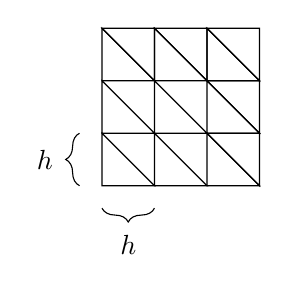
\begin{tikzpicture}
	\foreach \i in {0,...,2}
		\foreach \j in {0,...,2}
		{
			\pgfmathsetmacro{\xu}{\i / 3};
			\pgfmathsetmacro{\yu}{\j / 3};
			\pgfmathsetmacro{\xd}{(\i + 1)/ 3};
			\pgfmathsetmacro{\yd}{\j / 3};			
			\pgfmathsetmacro{\xt}{\i / 3};
			\pgfmathsetmacro{\yt}{(\j + 1)/ 3};
			\pgfmathsetmacro{\xq}{(\i + 1) / 3};
			\pgfmathsetmacro{\yq}{(\j + 1)/ 3};
			
			\draw (2*\xu,2*\yu)
			-- (2*\xd,2*\yd)
			-- (2*\xt,2*\yt)
			-- cycle;
			\ifthenelse{\i=2 \OR \j=2}{\draw (2*\xd,2*\yd) 
							-- (2*\xt,2*\yt)
							-- (2*\xq,2*\yq)
							-- cycle;}{}
	}
	\draw [decorate,decoration={brace,amplitude=5pt,mirror,raise=1pt},yshift=0pt]
	(0,-0.25) -- (2/3,-0.25) node [midway,below,yshift=-0.25cm] {$h$};
	\draw [decorate,decoration={brace,amplitude=5pt,mirror,raise=1pt},yshift=0pt]
	(-0.25,2/3) -- (-0.25,0) node [midway,left,xshift=-0.25cm] {$h$};
	\end{tikzpicture}
	& 
	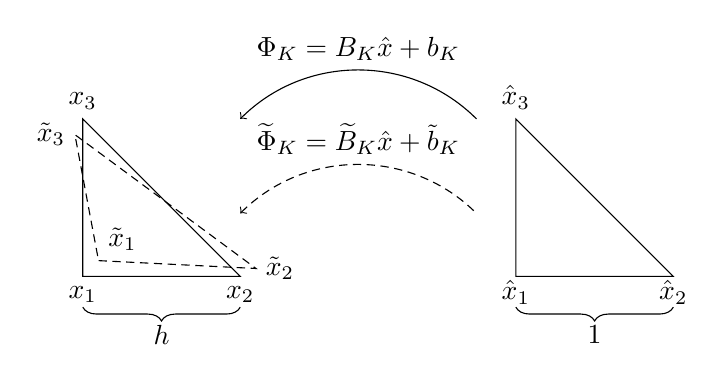
\begin{tikzpicture}
	\draw (0,0) node[anchor=north]{$x_1$}
	-- (2,0) node[anchor=north]{$x_2$}
	-- (0,2) node[anchor=south]{$x_3$}
	-- cycle;
	\draw[densely dashed] (0.2,0.2) node[anchor=south west]{$\tilde x_1$}
	-- (2.2,0.1) node[anchor=west]{$\tilde x_2$}
	-- (-0.1,1.8) node[anchor=east]{$\tilde x_3$}
	-- cycle;
	\draw[<-] (2, 2) to[out=45,in=135] node[above] {$\Phi_K = B_K \hat x + b_K$} (5, 2);
	\draw[<-, densely dashed] (2, 0.8) to[out=45,in=135] node[above] {$\btilde \Phi_K = \btilde B_K \hat x + \tilde b_K$} (5, 0.8);
	\draw (5.5,0) node[anchor=north,yshift=0.07cm]{$\hat x_1$}
	-- (7.5,0) node[anchor=north,yshift=0.07cm]{$\hat x_2$}
	-- (5.5,2) node[anchor=south]{$\hat x_3$}
	-- cycle;
	\draw [decorate,decoration={brace,amplitude=5pt,mirror,raise=4pt},yshift=0pt]
	(0,-0.25) -- (2,-0.25) node [midway,below,yshift=-0.25cm] {$h$};
	\draw [decorate,decoration={brace,amplitude=5pt,mirror,raise=4pt},yshift=0pt]
	(5.5,-0.25) -- (7.5,-0.25) node [midway,below,yshift=-0.25cm] {$1$};
	\end{tikzpicture}
	\end{tabular}
	\caption{Structured mesh in the two-dimensional case.}
	\label{fig:StrucMesh}
	\end{figure}

	\underline{2d structured mesh with constant mesh size $h$ and $\kappa(x) = 1$}
		
	Let us consider a two-dimensional square domain and a structured mesh with constant mesh size $h$, as the one of \cref{fig:StrucMesh}. The reference triangle $\bhat K$, with vertices $\hat x_1 = (0, 0)^\top$, $\hat x_2 = (1, 0)^\top$ and $\hat x_3 = (0, 1)^\top$ is transformed into any element $K$ of the mesh via an affine map $\Phi_K(\hat x) = B_K \hat x + b_K$. Likewise, the modified triangle $\btilde K$ is obtained from $\bhat K$ via a modified map $\btilde \Phi_K$, which is affine too and given by $\btilde \Phi_K(\hat x) = \btilde B_K \hat x + \tilde b_K$. For the structured mesh, the matrices $B_K$ are all equal alternatively to $B_K = hI$ or $B_K = -hI$, where $I$ is the identity in $\R^{2\times 2}$, while the translation vector $b_K$ depends on the position inside the mesh. In the following, we will consider a single element $K$ (respectively $\btilde K$ in the perturbed mesh) such that $B_K = hI$ and denote $B = B_K$ (respectively $\btilde B = \btilde B_K$). Moreover, we will call its vertices $x_1$, $x_2$ and $x_3$ (respectively $\tilde x_1$, $\tilde x_2$ and $\tilde x_3$). The matrix $\btilde B$ is given by
	\begin{equation}
	\begin{aligned}
		\btilde B &= \begin{pmatrix}\tilde x_2 - \tilde x_1 \mid \tilde x_3 - \tilde x_1\end{pmatrix} \\
		&= B + \Lambda h^{p+1},
	\end{aligned}
	\end{equation}
	where $\Lambda \in \R^{2\times 2}$ is defined as
	\begin{equation}
		\Lambda = \begin{pmatrix}\alpha_2 - \alpha_1 \mid \alpha_3 - \alpha_1\end{pmatrix}.
	\end{equation}
	We can then compute the local contributions to $a(\tilde \phi_i, \tilde \phi_j)$ via integrals on the reference triangle as
	\begin{equation}
	\begin{aligned}
		\int_{\btilde K} \nabla \tilde \phi_i \cdot \nabla \tilde \phi_j &= \int_{\bhat K} \btilde B \nabla \hat \phi_i \cdot \btilde B \nabla \hat \phi_j \frac{1}{\abs{\det\btilde B}} \\
		&= \frac{\abs{\bhat K}}{\abs{\det\btilde B}}(B + \Lambda h^{p+1})\nabla \hat \phi_i \cdot (B + \Lambda h^{p+1}) \nabla \hat \phi_j \\
		&=  R \frac{\abs{\bhat K}}{\abs{\det B}} B \nabla \hat \phi_i \cdot B \nabla \hat \phi_j \\
		&= R \int_K \nabla \phi_i \cdot \nabla \phi_j,
	\end{aligned}
	\end{equation}
	where $\hat \phi_i$ and $\hat \phi_j$ are the basis functions on the reference triangle corresponding to $\phi_i$ and $\phi_j$ and where
	\begin{equation}
		R = \frac{\abs{\det B}}{\abs{\det\btilde B}}\Big(1 + \frac{h^{p+1}(B\nabla \hat \phi_i \cdot \Lambda \nabla \hat \phi_j + B\nabla \hat \phi_j \cdot \Lambda \nabla \hat \phi_i) + h^{2p+2} \Lambda \nabla \hat \phi_i \cdot \Lambda \nabla \hat \phi_j}{B \nabla \hat \phi_i \cdot B \nabla \hat \phi_j}\Big),
	\end{equation}
	where $\hat \nabla \phi_i$ and $\hat \nabla \phi_j$ are not orthogonal. Being $B$ and $\Lambda$ in $\R^{2\times 2}$ and since $\det B = h^2$ and $B^{-1} = h^{-1} I$, it holds
	\begin{equation}
	\begin{aligned}
		\det \btilde B &= \det B + h^{2p+2} \det \Lambda + \det B \trace(B^{-1}\Lambda) h^{p+1} \\
			&= h^2 + h^{2p+2} \det \Lambda + \trace(\Lambda) h^{p+2}.
	\end{aligned}
	\end{equation}
	Hence, the ratio between the determinants is given by
	\begin{equation}
	\begin{aligned}
		\frac{\abs{\det B}}{\abs{\det\btilde B}} &= \frac{1}{\abs{1 + h^{2p} \det \Lambda + \trace(\Lambda) h^p}}\\
		&\leq 1 + \abs{(h^{2p} \det \Lambda + \trace(\Lambda) h^p)\big(1 + \sksum_{l=1}^\infty(-1)^l (h^{2p} \det \Lambda + \trace(\Lambda) h^p)^l\big)} \\
		&= 1 + C_1 h^p,
	\end{aligned}
	\end{equation}
	for the constant $C_1$ defined as
	\begin{equation}
		C_1 = \abs{(h^p \det \Lambda + \trace(\Lambda))\big(1 + \sksum_{l=1}^\infty(-1)^l (h^{2p} \det \Lambda + \trace(\Lambda) h^p)^l\big)},
	\end{equation}
	which is bounded independently of $h$. Moreover,
	\begin{equation}
	\begin{aligned}
		\frac{(B\nabla \hat \phi_i \cdot \Lambda \nabla \hat \phi_j + B\nabla \hat \phi_j \cdot \Lambda \nabla \hat \phi_i) }{B \nabla \hat \phi_i \cdot B \nabla \hat \phi_j}h^{p+1}
		&= 	\frac{(\nabla \hat \phi_i \cdot \Lambda \nabla \hat \phi_j + \nabla \hat \phi_j \cdot \Lambda \nabla \hat \phi_i)}{\nabla \hat \phi_i \cdot \nabla \hat \phi_j} h^p\\
		&= C_2 h^p,
	\end{aligned}
	\end{equation}
	where $C_2$ is bounded independently of $h$. Finally
	\begin{equation}
	\begin{aligned}
		\frac{\Lambda \nabla \hat \phi_i \cdot \Lambda \nabla \hat \phi_j}{B \nabla \hat \phi_i \cdot B \nabla \hat \phi_j}h^{2p+2} 
		&= \frac{\Lambda \nabla \hat \phi_i \cdot \Lambda \nabla \hat \phi_j}{\nabla \hat \phi_i \cdot \nabla \hat \phi_j}h^{2p} \\
		&= C_3 h^{2p},
	\end{aligned}
	\end{equation}
	where $C_3$ is bounded independently of $h$. Hence
	\begin{equation}
		\int_{\btilde K} \nabla \tilde \phi_i \cdot \nabla \tilde \phi_j - \int_K \nabla \phi_i \cdot \nabla \phi_j = \Big(\int_K \nabla \phi_i \cdot \nabla \phi_j\Big) C h^p,
	\end{equation}
	where 
	\begin{equation}
		C = C_1 + C_2 + C_1C_2h^p + C_3h^p + C_1C_3h^{2p},
	\end{equation}
	which proves the desired result.	
	
	\underline{2d mesh with $\kappa(x) = 1$}
	
%	Analogously as in the case of the structured mesh and choosing without loss of generality $x_1$ as the origin in $\R^2$, we have
%	\begin{equation}
%		\btilde B_K = B_K + \Lambda_K,
%	\end{equation}
%	where
%	\begin{equation}
%		\Lambda_K = \begin{pmatrix} \bar h_2^{p+1}\alpha_2 - \bar h_1^{p+1} \alpha_1 \mid \bar h_3^{p+1} \alpha_3 - \bar h_1^{p+1} \alpha_1\end{pmatrix}.
%	\end{equation}
%	Under \cref{as:MeshPerturbation}, the matrix $\Gamma_K$ satisfies element-wise $\abs{\Gamma_K} \leq C h^{p+1}$, where $C$ is a positive constant bounded independently of $h$. Repeating the computation as above, we find
%	\begin{equation}
%		\int_{\btilde K} \nabla \tilde \phi_i \cdot \nabla \tilde \phi_j = R_K \int_K \nabla \phi_i \cdot \nabla \phi_j,
%	\end{equation}
%	where
%	\begin{equation}
%		R_K = \frac{\abs{\det B_K}}{\abs{\det\btilde B_K}}\Big(1 + \frac{B_K\nabla \hat \phi_i \cdot \Gamma_K \nabla \hat \phi_j + B_K \nabla \hat \phi_j \cdot \Gamma_K \nabla \hat \phi_i + \Gamma_K \nabla \hat \phi_i \cdot \Gamma_K \nabla \hat \phi_j}{B_K \nabla \hat \phi_i \cdot B_K \nabla \hat \phi_j}\Big).
%	\end{equation}
%	The determinant of $\btilde B_K$ can be expressed as
%	\begin{equation}
%	\begin{aligned}
%		\det \btilde B_K &= \det B_K + \det \Gamma_K + \det B_K \trace(B_K^{-1}\Gamma_K) h^{p+1} \\
%		&= h^2 + h^{2p+2} \det \Lambda + \trace(\Lambda) h^{p+2}.
%	\end{aligned}
%	\end{equation}
%	
%	Let us consider an element $K \in \mathcal T_h$ with vertices $x_1$, $x_2$ and $x_3$. Without loss of generality, we fix $x_1 = 0 \in \R^2$. Let us then consider the perturbed element $\btilde K \in \btilde{\mathcal T}_h$ corresponding to $K$ and the affine mapping $\Psi_K(x) = T_K x + t_K$ such that $\Psi_K(K) = \btilde K$ and such that $\btilde \Phi_K = \Psi_K \circ \Phi_K$. Constraining the vertices of $K$ to be mapped into the vertices of $\tilde K$, one gets first
%	\begin{equation}
%		t_K = \tilde x_1 = \alpha_1 \bar h_1^{p+1}.
%	\end{equation}
%	Then, for the two other vertices,
%	\begin{equation}
%	\begin{aligned}
%		T_K x_2 &= \tilde x_2 - \alpha_1 \bar h_1^{p+1},\\
%		T_K x_3 &= \tilde x_3 - \alpha_1 \bar h_1^{p+1}.
%	\end{aligned}
%	\end{equation}
%	From the definition of $\tilde x_2$ and $\tilde x_3$, it is clear that $T_K = I + \Gamma_K$ where $\Gamma_K$ satisfies
%	\begin{equation}
%	\begin{aligned}
%		\Gamma_K x_2 &= \alpha_2 \bar h_2^{p+1}- \alpha_1 \bar h_1^{p+1}, \\
%		\Gamma_K x_3 &= \alpha_3 \bar h_3^{p+1}- \alpha_1 \bar h_1^{p+1}.
%	\end{aligned}
%	\end{equation}
%	Subtracting the two equations, we get
%	\begin{equation}
%		\Gamma_K (x_2 - x_3) = \alpha_2 \bar h_2^{p+1}- \alpha_3 \bar h_3^{p+1}, \\
%	\end{equation}
%	which can be expressed component-wise for $i = 1, 2$ as
%	\begin{equation}
%		(\Gamma_K)_{i,1} (x_2 - x_3)_1 + (\Gamma_K)_{i,2} (x_2 - x_3)_2 = (\alpha_2)_i \bar h_2^{p+1} - (\alpha_3)_i \bar h_3^{p+1}.
%	\end{equation}
%	Since $x_2$ and $x_3$ are linearly independent, for any vector $w \in \R^2$ such that $\norm{w}_{\R^2} \leq C < \infty$ for a constant $C > 0$ it is valid
%	\begin{equation}
%	\begin{aligned}
%		\norm{\Gamma_K w}_{\R^2} &\leq C \sum_{j=1}^3 \norm{\alpha_j}_{\R^2} h^{p+1} \\
%		&\leq C h^{p+1}.
%	\end{aligned}
%	\end{equation}
%	Furthermore, {\color{blue}it is possible to show} that the entries of $\Gamma_K$ satisfy $\abs{(\Gamma_K)_{i,j}} \leq C h^p$ for a constant $C > 0$ and for $i, j = 1, 2$. The matrix defining the transformation $\btilde \Phi_K$ is then given by $\btilde B_K = T_K B_K = (I + \Gamma_K) B_K$. Let us remark that equivalently to the structured mesh, it holds
%	\begin{equation}
%		\int_{\btilde K} \nabla \tilde \phi_i \cdot \nabla \tilde \phi_j = R_K \int_K \nabla \phi_i \cdot \nabla \phi_j,
%	\end{equation}
%	where $R_K$ is given by
%	\begin{equation}
%	\begin{aligned}
%		R_K = \frac{\abs{\det B_K}}{\abs{\det\btilde B_K}}\Big(1 &+ \frac{B_K\nabla \hat \phi_i \cdot \Gamma_K B_K \nabla \hat \phi_j + B_K\nabla \hat \phi_j \cdot \Gamma_K B_K \nabla \hat \phi_i}{B_K \nabla \hat \phi_i \cdot B_K \nabla \hat \phi_j} \\
%		&+ \frac{\Gamma_K B_K \nabla \hat \phi_i \cdot \Gamma_K B_K \nabla \hat \phi_j}{B_K \nabla \hat \phi_i \cdot B_K \nabla \hat \phi_j}\Big).
%	\end{aligned}
%	\end{equation}
%	Let us consider the ratio between determinants. From the definition of $\btilde B_K$ we have
%	\begin{equation}
%	\begin{aligned}
%		\det \btilde B_K &= \det B_K + \det (B_K \Gamma_K) + \det B_K \trace(B_K^{-1} \Gamma_KB_K)\\
%		&= \det B_K \big(1 + \det\Gamma_K + \trace(\Gamma_K)\big),
%	\end{aligned}
%	\end{equation}
%	where we exploited the properties of the determinant. Moreover, since the entries of $\Gamma_K$ are bounded by $Ch^p$, it is clear that $\trace(\Gamma_K) \leq Ch^p$ and an application of Hadamard's inequality yields $\det \Gamma_K \leq Ch^{2p}$. Hence, 
%	\begin{equation}
%	\begin{aligned}
%		\frac{\abs{\det B_K}}{\abs{\det\btilde B_K}} &= \frac{1}{\abs{1 + C(h^{2p} + h^p)}}\\
%		&\leq 1 + C h^p.
%	\end{aligned}
%	\end{equation}
%	{\color{red} Prove lower bound for denominator}. Hence
%	\begin{equation}
%		\frac{B_K\nabla \hat \phi_i \cdot \Gamma_K B_K \nabla \hat \phi_j + B_K\nabla \hat \phi_j \cdot \Gamma_K B_K \nabla \hat \phi_i}{B_K \nabla \hat \phi_i \cdot B_K \nabla \hat \phi_j} \leq C h^p.
%	\end{equation}
	
	Let us now prove \eqref{eq:Lemma1Eq2}. Denoting by $\mathbf{w_h}$ and $\mathbf{v_h}$ the vector of the nodal values of $w_h$ and $v_h$ respectively, we have
	\begin{equation}
	\begin{aligned}
		\delta a(w_h, v_h) &= \sum_{i,j} (\mathbf{w_h})_i(\mathbf{v_h})_j \delta a(\phi_i, \phi_j)\\
		&\leq Ch^p \sum_{i,j} (\mathbf{w_h})_i(\mathbf{v_h})_j a(\phi_i, \phi_j)\\
		&\leq CMh^p \norm{w_h}_V \norm{v_h}_V,
	\end{aligned}
	\end{equation}
	where we applied \eqref{eq:Lemma1Eq1} and the continuity of $a$ to get the desired result.
\end{proof}

\begin{remark} Perturbation on the mesh is equivalent in algebraic formulation to a perturbation on the stiffness matrix $A$, as \eqref{eq:Lemma1Eq1} yields
	\begin{equation}
		\btilde A_{i,j} = A_{i,j} + C_{i,j} h^p.
	\end{equation}
	If the $C_{i,j}$ can be written explicitly given the $\alpha_i$, the stiffness matrix $\btilde A_{i,j}$ does not have to be assembled for each perturbation of the mesh.
\end{remark}

\begin{lemma}\label{lem:F} Under \cref{as:MeshPerturbation}, there exists a constant $C_F > 0$ independent of $h$ such that
	\begin{equation}
	\abs{F(P_h^{-1} v_h - v_h)} \leq C_F h^{p+1} \norm{v_h}_V,
	\end{equation}
	for all $v_h \in V_h$.
\end{lemma}
\begin{proof} \todo
\end{proof}

\begin{lemma}\label{lem:uHatU} Under \cref{as:MeshPerturbation}, let $\hat u_h \in \btilde V_h$ be the unique solution of
\begin{equation}
	a(\hat u_h, P_h^{-1}v_h) = F(v_h), 
\end{equation}
for all $v_h \in V_h$. Then, if $\bhat U_h = P_h \hat u_h$,
\begin{equation}
	\norm{\bhat U_h - u_h}_V \leq C \norm{\bhat U_h}_V h^p \quad \text{a.s. in } \Omega,
\end{equation} 
where $C > 0$ is a constant independent of $h$.
\end{lemma}
\begin{remark} Existence and uniqueness of $\hat u_h$ guaranteed as \dots
\end{remark}
\begin{proof}
For any $w_h, v_h \in V_h$ 
\begin{equation}\label{eq:defDeltaA}
	a(P_h^{-1} w_h, P_h^{-1} v_h) = a(w_h, v_h) + \delta a(w_h, v_h),
\end{equation}
where $\delta a(w_h, v_h) = a(P_h^{-1} w_h, P_h^{-1} v_h) - a(w_h, v_h)$. From the definition of $\hat u_h$ and $\bhat U_h$, we have for all $v_h \in V_h$
\begin{equation}
	a(P_h^{-1}\bhat U_h, P_h^{-1} v_h) = F(v_h),
\end{equation}
which can be rewritten thanks to \eqref{eq:defDeltaA} as
\begin{equation}
	a(\bhat U_h, v_h) + \delta a(\bhat U_h, v_h) = F(v_h).
\end{equation}
Subtracting $a(u_h, v_h)$ on both sides gives
\begin{equation}
	a(u_h - \bhat U_h, v_h) = \delta a(\bhat U_h, v_h).
\end{equation}
By the coercivity of $a$ and thanks to \cref{lem:DistATildaA} we then have, defining $\hat \epl_h = u_h - \bhat U_h$ and choosing $v_h = \hat \epl_h$,
\begin{equation}
	\alpha \norm{\hat \epl_h}_V^2 \leq Ch^p \norm{\hat U_h}_V \norm{\hat \epl_h}_V,
\end{equation}
which gives the desired result dividing both sides by $\alpha \norm{\hat \epl_h}_V$.
\end{proof}
\begin{lemma}\label{lem:tildeUhatU} Under \cref{as:MeshPerturbation}, let $\tilde u_h \in \btilde V_h$ be the unique solution of
	\begin{equation}
		a(\tilde u_h, \tilde v_h) = F(\tilde v_h), 
	\end{equation}
	for all $\tilde v_h \in \btilde V_h$. Then, if $U_h = P_h \tilde u_h$ and $h$ is sufficiently small
	\begin{equation}
		\norm{U_h - \hat U_h}_V \leq C h^{p+1} \quad \text{a.s. in } \Omega,
	\end{equation} 
	where $C > 0$ is a constant independent of $h$.
\end{lemma}
\begin{proof} Thanks to the definition of $\tilde u_h$ and $\hat u_h$, we have for all $v_h \in V_h$
	\begin{equation}
		a(P_h^{-1} U_h - P_h^{-1} \bhat U_h, P_h^{-1} v_h) = F(P_h^{-1} v_h - v_h).
	\end{equation}	
	Thanks to \eqref{eq:defDeltaA} and the linearity of $P_h^{-1}$, we then obtain
	\begin{equation}
		a(U_h - \bhat U_h, v_h) = F(P_h^{-1} v_h - v_h) - \delta a(U_h - \bhat U_h, v_h).
	\end{equation}
	Exploiting the coercivity of $a$, introducing the notation $\epl_h = U_h - \bhat U_h$ and choosing $v_h = \epl_h$, we get
	\begin{equation}
		\alpha \norm{\epl_h}_V^2 \leq F(P_h^{-1} \epl_h - \epl_h) - \delta a(\epl_h, \epl_h).
	\end{equation}
	Let us consider the two terms on the right hand side separately. For the first term we apply directly \cref{lem:F} and for the second term we apply \cref{lem:DistATildaA}, thus obtaining
	\begin{equation}
		\alpha \norm{\epl_h}_V^2 \leq C_F h^{p+1} \norm{\epl_h}_V + C \norm{\epl_h}_V^2,
	\end{equation}
	where $C$ is given in \cref{lem:DistATildaA}. Dividing both sides by $\norm{\epl_h}_V$ we finally get
	\begin{equation}
		(\alpha - C) \norm{\epl_h}_V \leq C_Fh^{p+1}. 
	\end{equation}
	Hence, if $h$ satisfies
	\begin{equation}
		h < \Big(\frac{\alpha}{C}\Big)^{1/p},
	\end{equation}
	we obtain the desired result.
\end{proof}
\begin{theorem} Under \cref{as:MeshPerturbation}, 
	\begin{equation}
		\norm{U_h - u_h}_V \leq C h^p \quad \text{a.s. in } \Omega,
	\end{equation}
	where $C > 0$ is a constant independent of $h$.
\end{theorem}

\begin{proof} The triangular inequality yields
	\begin{equation}
	\begin{aligned}
	\norm{U_h - u_h}_V &\leq \norm{U_h - \hat U_h}_V + \norm{\hat U_h - u_h}_V \\
	&\leq C_1 h^p + C_2 h^{p+1},
	\end{aligned} 
	\end{equation}
	where we applied \cref{lem:tildeUhatU} and \cref{lem:uHatU}.
\end{proof}

\begin{theorem} Under \cref{as:MeshPerturbation}, 
	\begin{equation}
		\norm{U_h - u}_V \leq C h \quad \text{a.s. in } \Omega,
	\end{equation}
	where $C > 0$ is a constant independent of $h$.
\end{theorem}

\begin{proof} The triangular inequality and the standard convergence analysis of the finite elements method yields
	\begin{equation}
	\begin{aligned}
		\norm{U_h - u}_V &\leq \norm{U_h - u_h}_V + \norm{u - u_h}_V \\
		&\leq C_1 h^p + C_2 h,
	\end{aligned} 
	\end{equation}
	which gives the desired result since $p \geq 1$.
\end{proof}

\section{A posteriori error analysis}
\section{Mesh adaptivity}
\section{Inverse problems}

\section{Numerical experiments}

\subsection{Convergence}

\subsection{Error estimators}

\subsection{Mesh adaptivity}



\bibliographystyle{siamplain}
\bibliography{anmc}
\end{document}